 
\chapter{Dados Obtidos}
\label{cap6}
%ccm Não esquecer de zerar o eixo X
%ccm todo gráfico precisa responder a alguma pergunta.
% 1- Formular a pergunta com base no que definiu no Cap.4
% 2- quem está envolvido, quais são os parâmetros, quais são constantes
% 3- Descrever o perfil/modus operandi do experimento
% 4- Mostra a figura
% 5- Analisa os resultados com base na expectativa no Cap.4 (foi similar, diferente, por quê?)
% 6 - Precisa manter em mente que as figuras devem manter uma escala para poder comparar entre diferentes arquiteturas




\begin{figure}[htb!]
    \caption{Tempo de requisição a partir dos Clientes}
    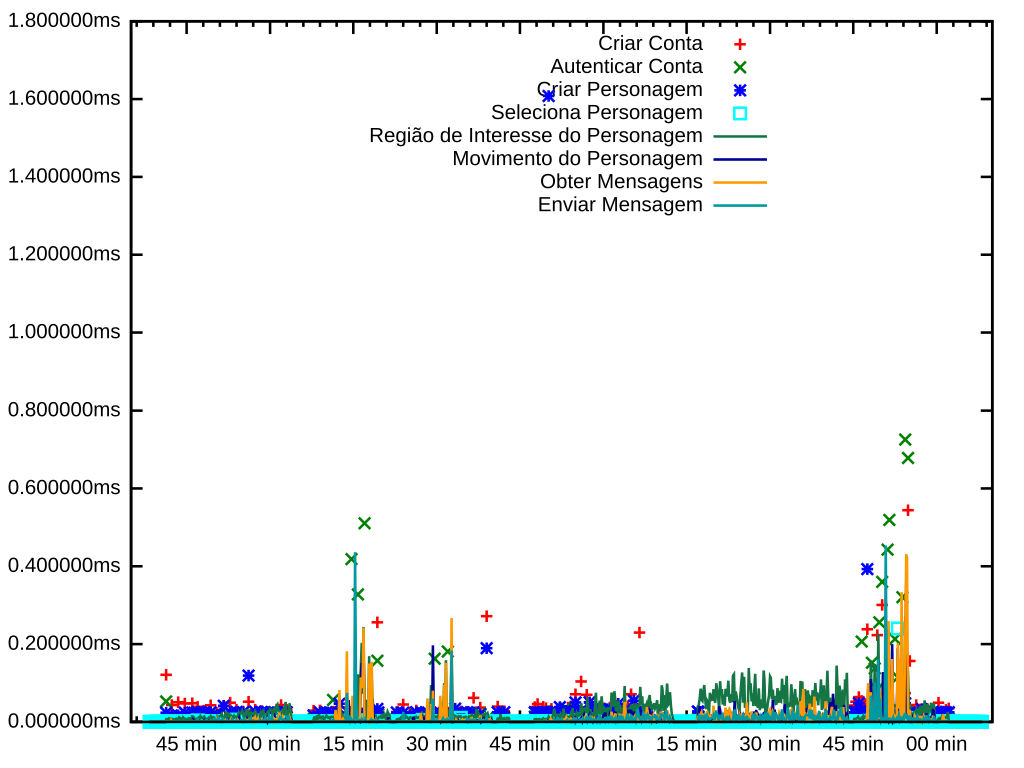
\includegraphics[width=\textwidth]{metricas_rudy_t3/rudyc.png}
    \centering
    
    Fonte: O próprio autor
\end{figure}

\begin{figure}[htb!]
    \caption{Tempo de requisição a partir dos Clientes}
    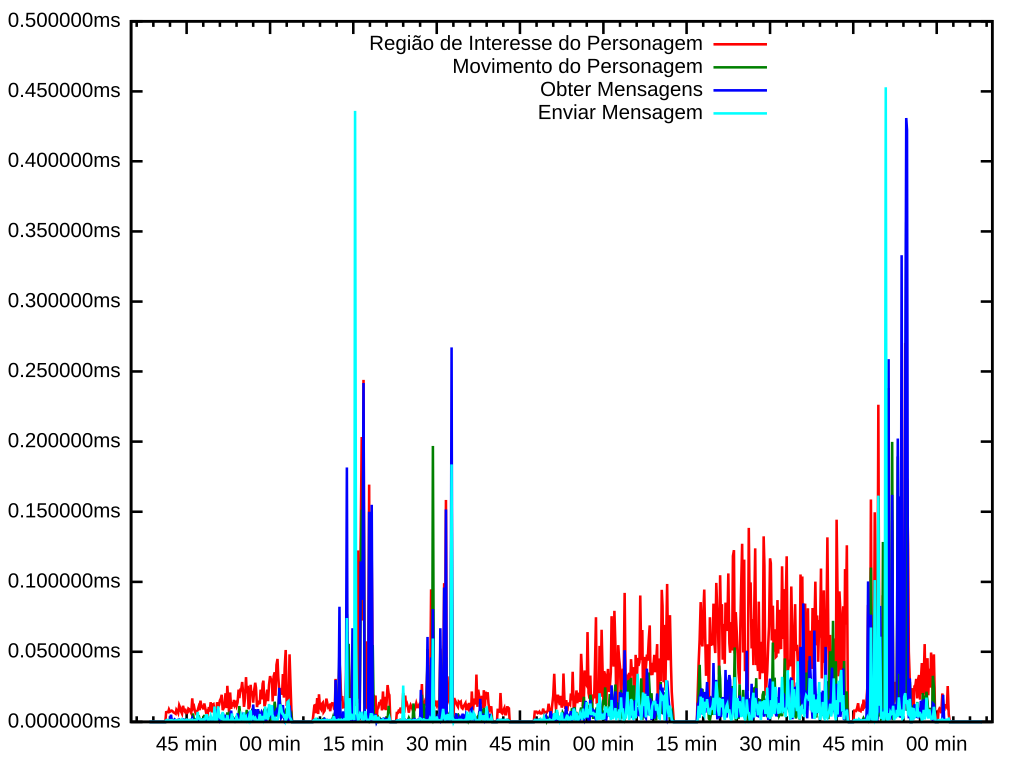
\includegraphics[width=\textwidth]{metricas_rudy_t3/rudyc_rpc.png}
    \centering
    
    Fonte: O próprio autor
\end{figure}

\begin{figure}[htb!]
    \caption{Tempo de requisição a partir dos Clientes}
    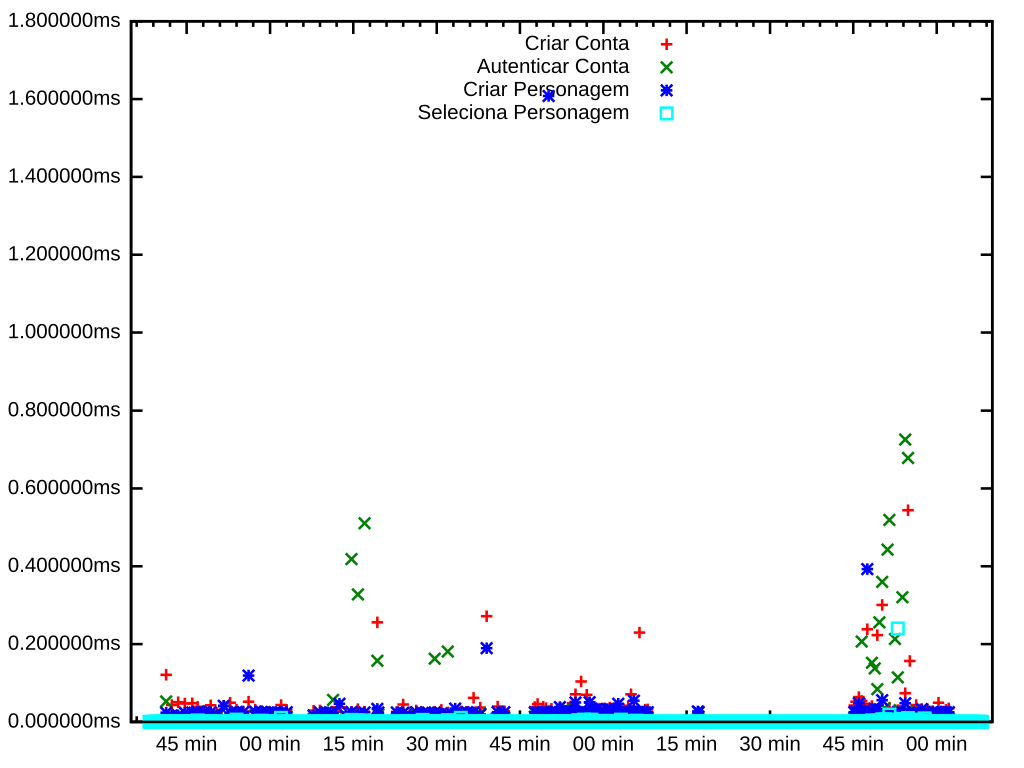
\includegraphics[width=\textwidth]{metricas_rudy_t3/rudyc_http.png}
    \centering
    
    Fonte: O próprio autor
\end{figure}

\begin{figure}[htb!]
    \caption{Tempo de requisição a partir dos Clientes}
    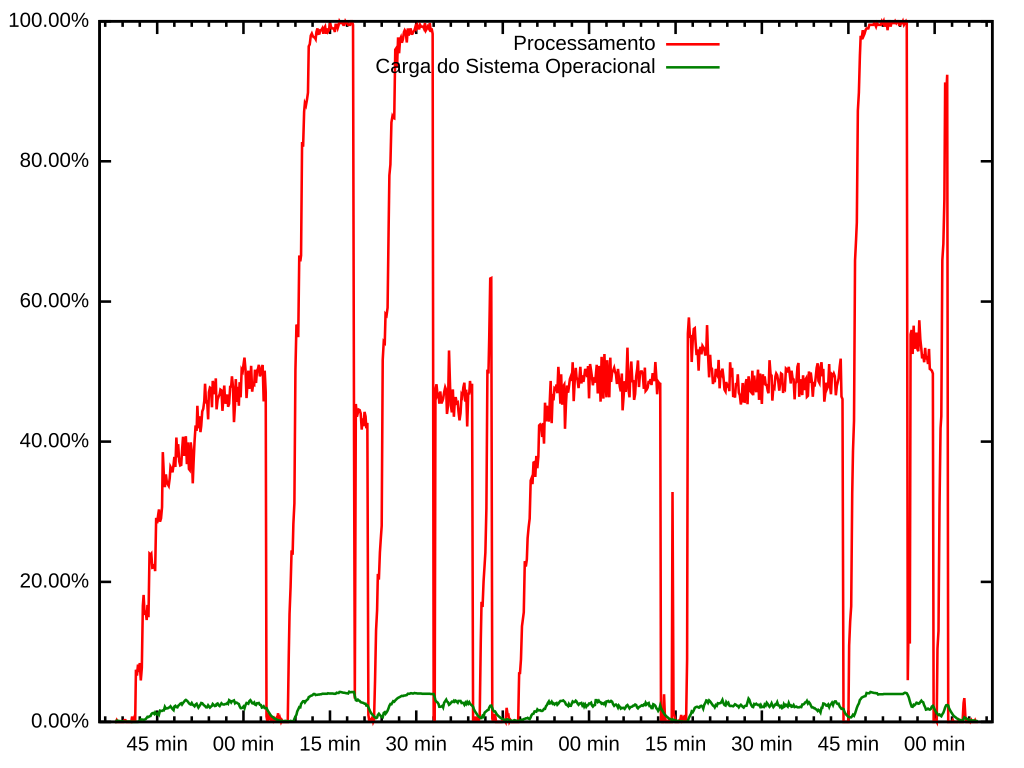
\includegraphics[width=\textwidth]{metricas_rudy_t3/cpu.png}
    \centering
    
    Fonte: O próprio autor
\end{figure}

\begin{figure}[htb!]
    \caption{Tempo de requisição a partir dos Clientes}
    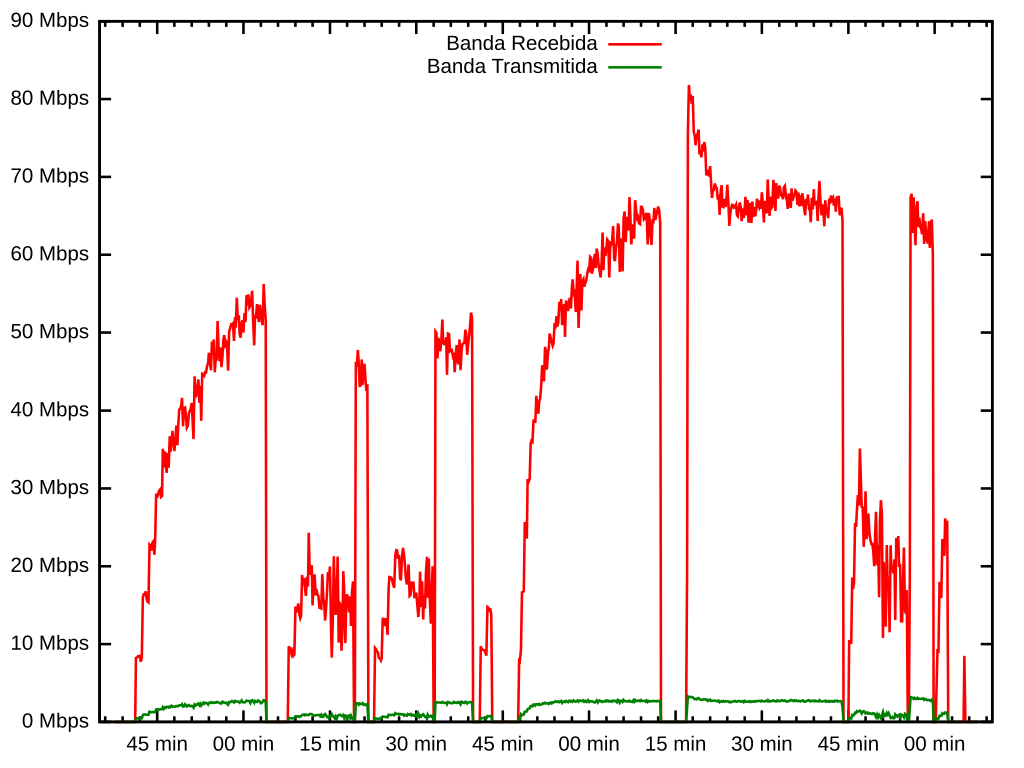
\includegraphics[width=\textwidth]{metricas_rudy_t3/io.png}
    \centering
    
    Fonte: O próprio autor
\end{figure}

\begin{figure}[htb!]
    \caption{Tempo de requisição a partir dos Clientes}
    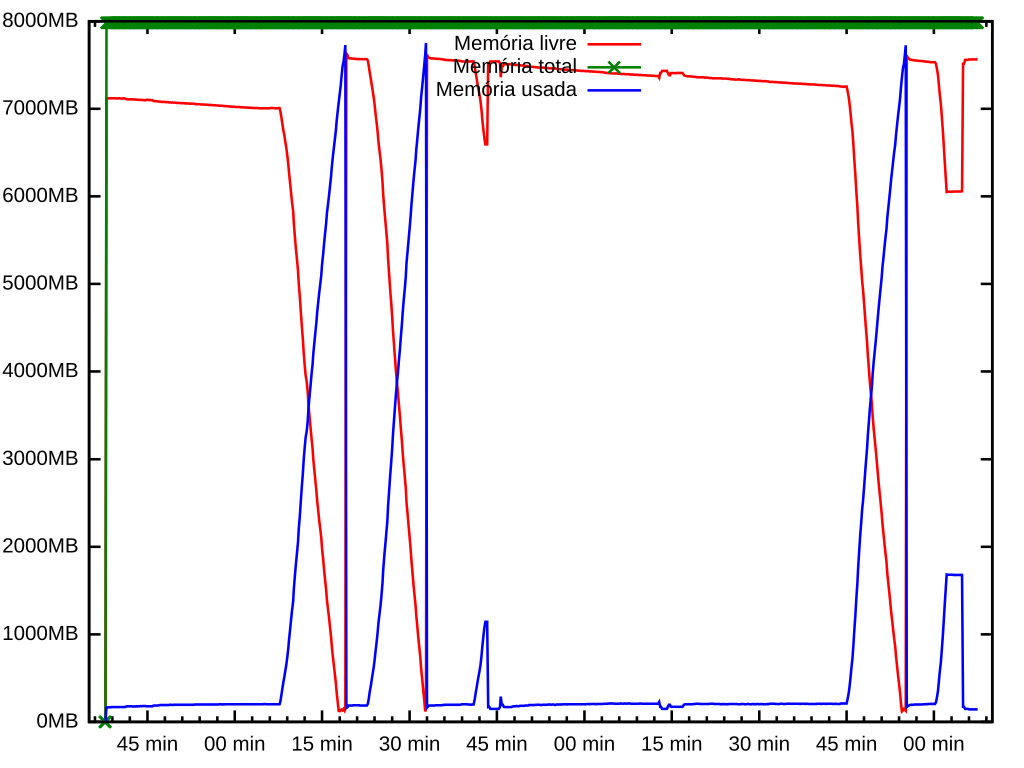
\includegraphics[width=\textwidth]{metricas_rudy_t3/memory.png}
    \centering
    
    Fonte: O próprio autor
\end{figure}
